	\chapter{Análise de resultados e validação}
	\label{cap:analise_de_resultados}
		
	O documento de Concepção do Sistema, entregue na Etapa 1 do MeDSE (Capítulo~\ref{cap:desenvolvimento}), contém os Requisitos Iniciais e o cenário que foi montado para a realização da experimentação (Capítulo~\ref{cap:estudo_de_caso}). A partir dos Requisitos Iniciais, foram processados seguidos refinamentos que culminaram na elaboração do projeto de sistema. O projeto de sistema foi transformado em simulações que foram transformadas em protótipos, e esses foram testados e validados, modular e sistemicamente, contra as especificações técnicas e requisitos. O estudo de caso realizou três pedidos de clientes. Essa realização produziu os resultados que são analisados neste capítulo.
		
	Duas seções são utilizadas para processar a análise e a validação. Na primeira seção é elaborado um modelo estático, contudo mais detalhado da produção de um produto usando os recursos do SIAPE. Esse exemplo de produção é usado conjuntamente com os resultados da experimentação para evidenciar que as restrições, os requisitos e as capacidades constantes na Tabela \ref{T14}, foram alcançadas evidenciando a validação do SIAPE contra os requisitos propostos.
			
	Na segunda seção esse mesmo modelo é utilizado para evidenciar comparações de performance contra o sistema denominado de Produto UFAM que serviu de base para o desenvolvimento do Produto SIAPE. A partir das comparações são realizadas algumas discussões em torno dos resultados para concluir a validação do SIAPE como um sistema evolutivo.  
	%=========================================================================================================	
		
					\begin{table}[!h]
						\centering
						\caption{	SIAPE - REQUISITOS / RESTRIÇÕES /CAPACIDADES		}
						\begin{tabular}{ |c | p{4cm}| p{6cm}|c| } \hline
							\textbf{Item} 	   & \textbf{Tipo} &\textbf{ Descrição} & \textbf{Código}\\ \hline
							
							01   & Restrição & tensão DC1 & RS01 \\ \hline
							02   & Restrição & corrente DC & RS02 \\ \hline
							03   & Restrição & Força módulo - elétrica & RS03 \\ \hline
							04   & Cliente-Performance & ciclo de produção mínimo & RQ01 \\ \hline
							05   & Cliente-Performance & setup simplificado  & RQ02 \\ \hline
							06   & Cliente-Performance & ramp up mínimo & RQ03 \\ \hline
							07   & Cliente-Performance &  lead time mínimo& RQ04 \\ \hline
							08   & Cliente-Produto Ufam & carimbar A,F,M,T,U & RQ05 \\ \hline
							09   & Cliente-Produto Ufam & carimbar palavra a partir do RQ5 & RQ06 \\ \hline
							10   & Interno-EPS & modularidade & RQ07 \\ \hline
							11   & Interno-EPS & plugabilidade & RQ08 \\ \hline
							12   & Interno-EPS & reconfigurabilidade & RQ09 \\ \hline
							13   & Enterno-Globalização & Customização & RQ10 \\ \hline
							14   & Externo-Governo & NR-12 (Segurança) & RQ11 \\ \hline
							15   & Externo-Economia & Custos & RQ12 \\ \hline
							16   & Externo-IoT & Plug \& Work & RQ13 \\ \hline
							17   & Externo-i4.o & Integração Horizontal & RQ14 \\ \hline
							18   & Externo-Academia & Estado da arte & RQ15 \\ \hline
						\end{tabular}												
						\label{T14}\par
						%	Fonte: Hiram Amaral
					\end{table}
		Como forma de organizar a análise a sequência da Tabela \ref{T14} é seguida, e cada tipo de requisito é tratado conforme a separação definida a seguir:  
		
		\begin{description}
		\item[Análise de resultado para os requsitos de RQ1 a RQ6 e restrições de RS1 a RS3] -
	Essa análise evidencia o atendimento das necessidades do cliente expressos pelos requisitos RQ1 a RQ6 e restrições RS1 a RS3. Com a expansão da análise consegue-se evidenciar que os objetivos específicos da proposta de pesquisa também foram atendidos. Isso,  quando se  enquadra a realização do sistema  como prova de conceito, tanto do método de desenvolvimento utilizado, quanto da funcionalidade do SIAPE. Considerando essa abordagem, os requisitos RQ1 a RQ6 e as restrições RS01 a RS03 - identificados na Tabela \ref{T14} - são discutidos em maior profundidade.\par
		
		\item[Análise de resultado para os requisitos de RQ7 a RQ12 e capacidades de CP1 a CP3] -
	Aqui, a questão recorrente do problema da customização em massa é tratada pelas principais capacidades dos sistemas evolutivos: capacidade de se adaptar e a capacidade de evoluir. Juntam-se às capacidades, as principais propriedades dos sistemas evolutivos para tratar o problema recorrente da customização de uma forma robusta que proporcione os níveis de competitividades para os produtos produzidos por esses tipos de sistemas. Essa análise envolve os requisitos RQ07 a RQ12, conforme descritos na Tabela \ref{T14}.
			
		\item[Análise de resultado para os requisitos de RQ13 a RQ15] -
	  Essa análise objetiva evidenciar a relação próxima que tem o estado da arte em paradigmas de produção, aqui considerado o paradigma evolutivo com a fronteira do conhecimento, aqui consideradas a Internet das Coisas e a Indústria 4.0 conforme descrito na Tabela \ref{T14}. 
		\end{description} 
			
	Antes de iniciar o processo de análise torna-se necessário relembrar alguns conceitos já mencionados nos Capítulos 1 e 2. A Figura \ref{F6} foi refeita convenientemente na horizontal e está ilustrada na Figura \ref{F118}. Esta figura identifica as fases do ciclo de vida do produto. Relembrando as fases do ciclo de vida do produto na fase 1, a equipe de marketing (MKT) realiza pesquisas para identificar as demandas não atendidas. Na Fase 2, a Engenharia de Desenvolvimento (END) transforma as necessidades não atendidas em produto a ser produzido; a área de Suprimentos (SUP) realiza a compra e a logística dos insumos necessários para a realização do produto; a Engenharia de Processo (ENP) na Fase 4, prepara o produto para ser aplicado às linhas de produção; a Produção acontece nas linhas de produção - que são desenvolvidas a partir de sistemas  de Engenharia e de Computação usando métodos da Automação Industrial (foco da análise deste capítulo); a área de Vendas e Distribuição (VDI) realiza as vendas e distribui os produtos no Comércio; a área de Instalação e Operações (IOP) realiza a instalação do produto e outras operações junto ao cliente;  a Assistência Técnica (ATD) dá suporte ao cliente e ajuda no descarte após a finalização do ciclo de vida do produto.  
	
					\begin{figure}[h]
						\centering
						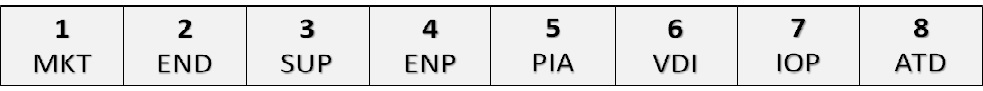
\includegraphics[width=16cm, height=1cm]{F118_CICLO_SIAPE.jpg} 
						\caption{SIAPE - Ciclo de vida do produto}
						\label{F118}
					\end{figure}
					
\section{Análise de resultados das  restrições, requisitos e capacidades}
		
A partir do ciclo de vida do produto, a fase de produção é explodida para facilitar o entendimento da análise dos resultados. Os componentes do sistema estão identificados, conforme pode ser visualizado na Figura \ref{F120}, foram explicados no Capítulo 2, e são utilizados na análise de cada tipo de requisito nesta subseção.  											
					
	
						\begin{figure}[h]
							\centering
							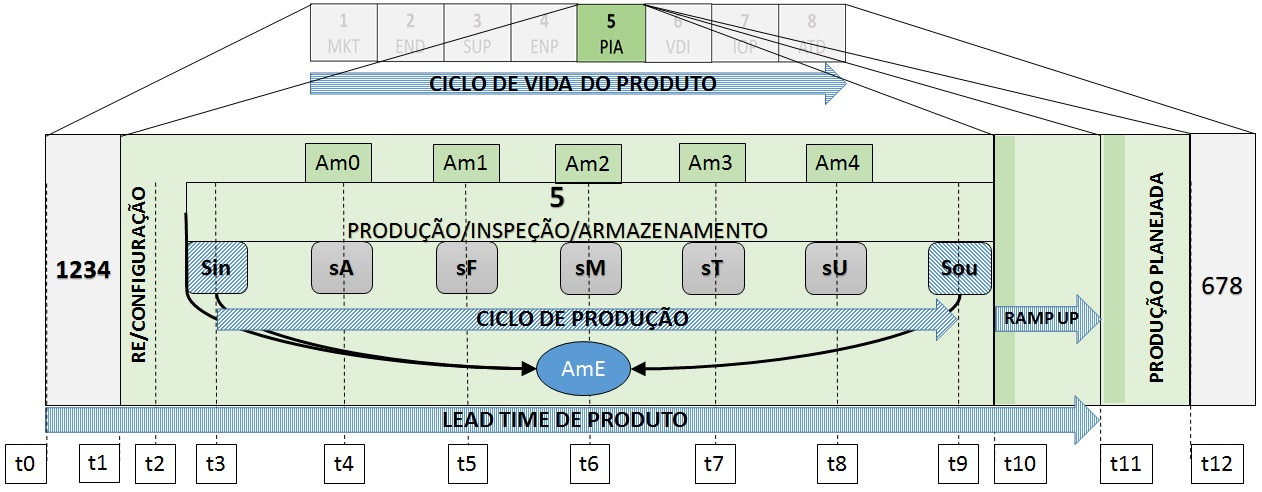
\includegraphics[width=16cm, height=6cm]{F120_SIAPE_CICLO_EXPLODIDO.jpg} 
							\caption{Ciclo de vida do produto: Fase Produção}
							\label{F120}
						\end{figure}
						
As fases iniciais do ciclo de vida do produto (1234) preparam as atividades da fase de produção, isto é, quando o operador recebe o pedido para ser processado, o SIAPE já está realizado tanto na parte de software quanto na parte de hardware. Essas fases acontecem entre t0 e t1. \par 

É plenamente compreensível para o leitor entender que entre os tempos (ti) podem ou não haver interrupções no processo que aqui não são consideradas.\par 

Quando o operador recebe o pedido de produção, em t1, o SIAPE é configurado e a linha alimentada. Em t2 o operador inicializa a esteira que carrega o palete na direção dos módulos. O agente acesso hardware que monitora os módulos presentes no sistema já tem informado ao OrderAgent todos os módulos do sistema. O OrderAgent por sua vez já incluiu no plano os recursos (letras) solicitadas pelo operador durante a configuração do plano de produção. Caso o recurso faça parte de um dos produtos solicitados, a esteira é movida exatamente para o local do recurso. O Stamper por sua vez realiza seu skill carimbar letra para imprimir a letra sobre o papel que encontra-se no palete. Uma vez carimbada a letra, a esteira é movida para o próximo recurso constante no plano de produção.\par 
O processo se repete até que o produto esteja totalmente produzido (a palavra completamente impressa no papel)  e o sensor de saída (Sou), no tempo t9,  identifique o palete e registre sua saída do ciclo de produção. De t1 até t9 são percorridas todas as operações de produção necessárias para a realização de uma unidade de produto. De t9 a t10 o produto é armazenado. No período compreendido entre os tempos t10 e t11 encontram-se as atividades relativas à curva de crescimento (ramp up), e de t11 a t12, o período de produção normal, onde todos os recursos de produção estão ajustados e atingiram a produção planejada. As áreas (678) que envolvem a área de Vendas e Distribuição (VDI), a área de Instalação e Operações (IOP) e a Assistência Técnica não são consideradas nestas análises. A Figura   \ref{F120_2} relaciona a Figura \ref{F6} com a Figura \ref{F120} para facilitar o entendimento do conceito de lead time.
	
		
		\begin{figure}[h]
			\centering
			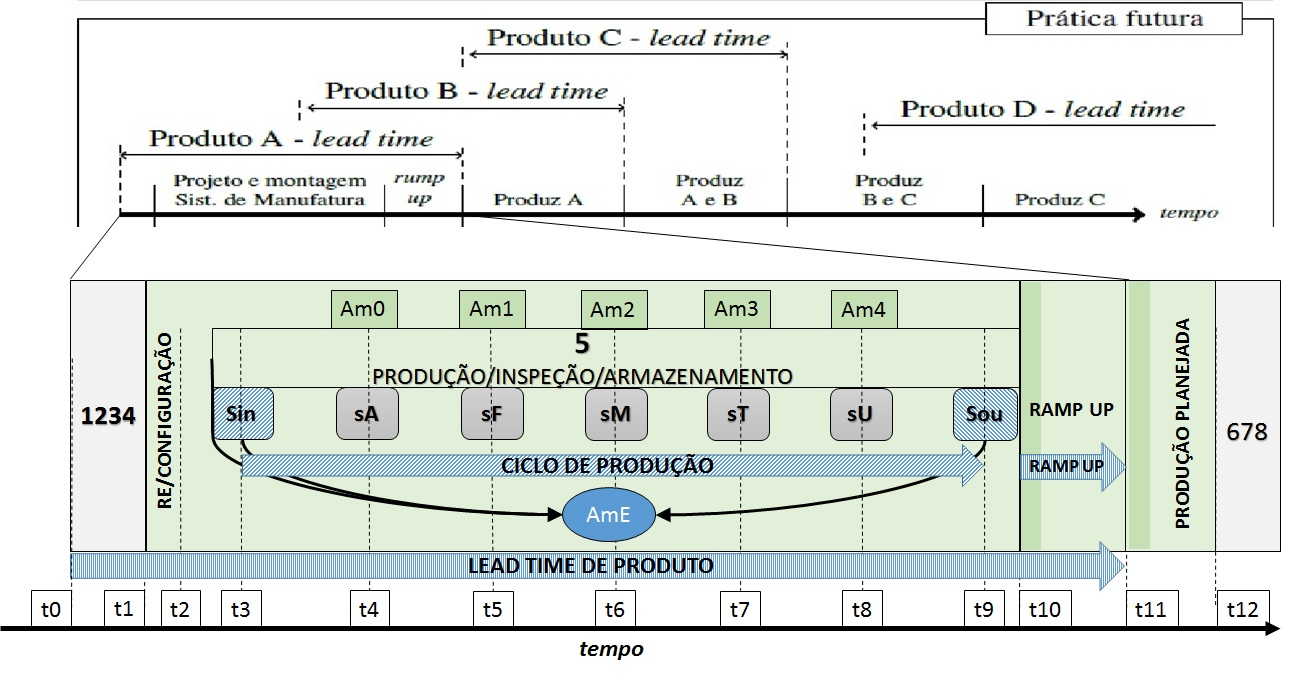
\includegraphics[width=16cm, height=6cm]{F120_2_SIAPE_CICLO_EXPLODIDO.jpg} 
			\caption{Ciclo de vida do produto: Lead time.}
			\label{F120_2}
		\end{figure}
	
A Figura \ref{F121} ilustra o palete de produção. Quatro posições são codificadas lateralmente no corpo do palete. A localização exata de uma letra é realizada pela posição primeiramente do módulo (Am0 a Am4) e depois pela posição codificada no palete (p1 a p4).
	
		\begin{figure}[h]
			\centering
			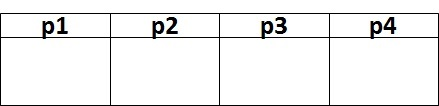
\includegraphics[width=7cm, height=1.5cm]{F121_SIAPE_PALETE.jpg} 
			\caption{SIAPE- Palete}
			\label{F121}
		\end{figure}
		
O exemplo a seguir produz um anagrama de quatro letras (A, F, M, U) para realizar a palavra UFAM e deve ser acompanhado pela Figura \ref{F123} que ilustra passo-a-passo o processo de produção para uma palavra processando o seguinte \textit{skill}: 
		
		Letra: A | MoveTo(0, 3) | stamp('A')
		Letra: F | MoveTo(1, 2) | stamp('F')
		Letra: M | MoveTo(2, 4) | stamp('M')
		Letra: U | MoveTo(4, 1) | stamp('U')
		
Para carimbar a letra A:  primeiro o palete é movido:
\begin{center}
	\textbf{Letra: A | MoveTo(0, 3)}
\end{center}
implicando que a esteira levará o palete para a posição (0) que corresponde ao módulo A, e o atuador do módulo A (Am0) carimbará a letra A na posição p3 (3) do palete. 

Essa operação\textbf{(1-Carimba A)}) ocorre no tempo t4, e o processo de detecção - quando necessário - é realizado pelo sensor do módulo A(sA), conforme ilustrado na Figura \ref{F123}

	\begin{figure}[!h]
		\centering
		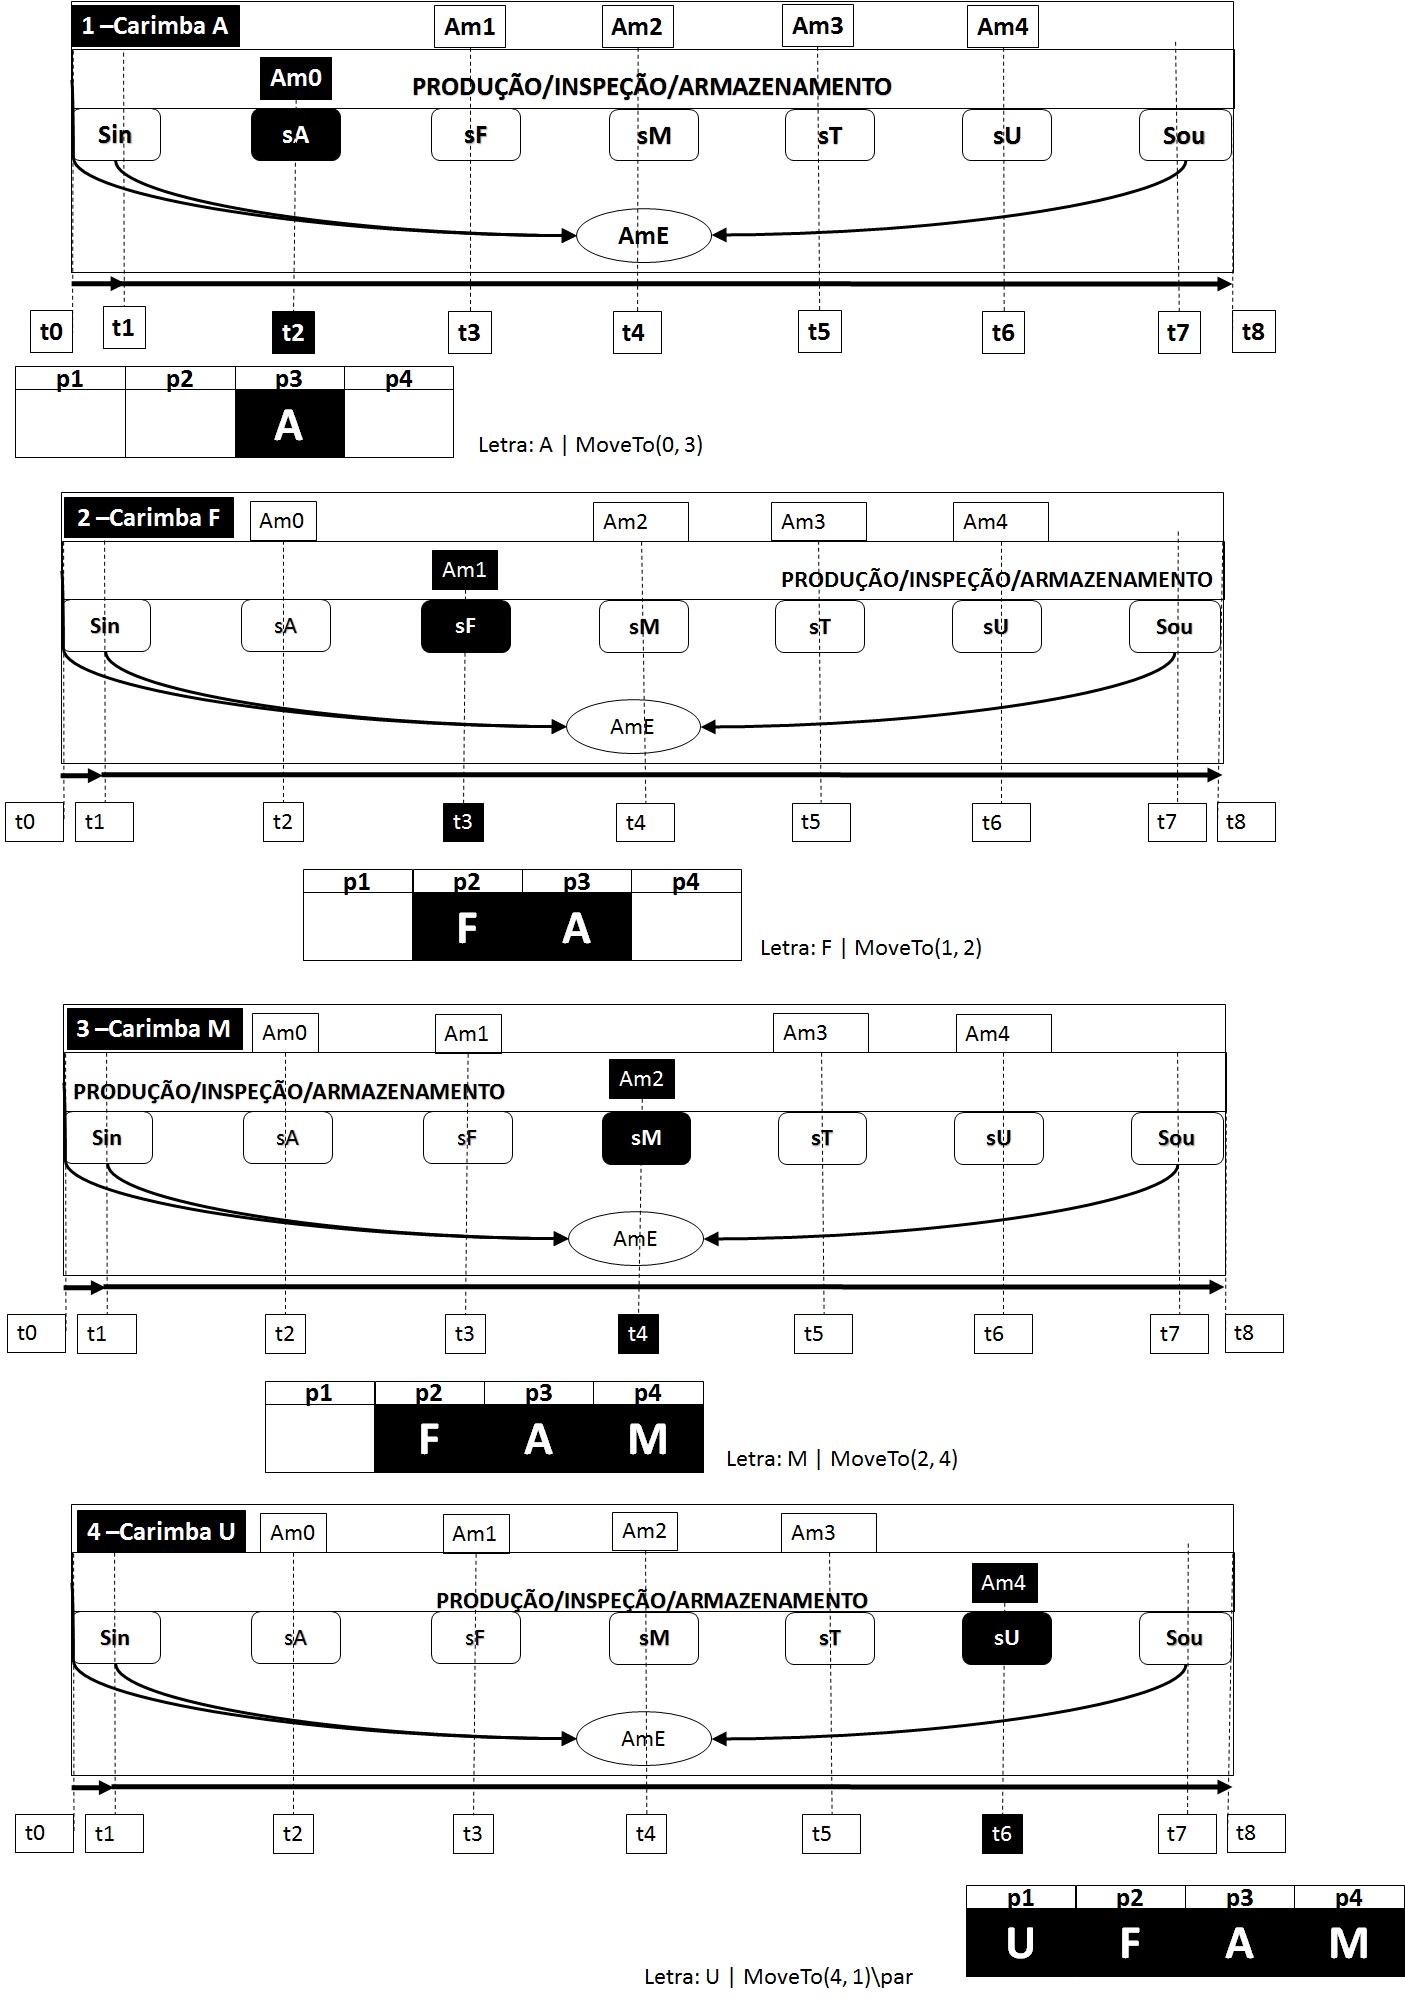
\includegraphics[width=16cm, height=22.5cm]{F123_PALAVRA_UFAM.jpg} 
		\caption{SIAPE- ANAGRAMA UFAM}
		\label{F123}
	\end{figure}

Para carimbar a letra F:  primeiro o palete é movido:
\begin{center}
	\textbf{Letra: F | MoveTo(1, 2)}
\end{center}
implicando que a esteira levará o palete para a posição (1) que corresponde ao módulo F, e o atuador do módulo F (Am1) carimbará a letra F na posição (2) do palete. 

Essa operação \textbf{(2-Carimba F)} ocorre no tempo t5, e o processo de detecção - quando necessário - é realizado pelo sensor do módulo F(sF), conforme ilustrado na Figura \ref{F123}.


Para carimbar a letra M: primeiro o palete é movido:
\begin{center}
	\textbf{Letra: M | MoveTo(2, 4)}
\end{center}
implicando que a esteira levará o palete para a posição (2) que corresponde ao módulo M, e o atuador do módulo M (Am2) carimbará a letra M na posição (4) do palete. 

Essa operação \textbf{(3-Carimba M)} ocorre no tempo t6, e o processo de detecção é realizado pelo sensor do módulo M(sM), conforme ilustado na Figura \ref{F123}; 

Para carimbar a letra U. Essa é movida para a seguinte posição
\begin{center}
\texttt{Letra: U | MoveTo(1, 2)}
\end{center}
implicando que a esteira levará o palete para a posição (4) que corresponde ao módulo U, e o atuador do módulo U (Am4) carimbará a letra U na posição (1) do palete. 

Essa operação \textbf{(4-Carimba U)} ocorre no tempo t8, e o processo de detecção é realizado pelo sensor do módulo U(sU), conforme ilustrado na Figura \ref{F123};

		
\subsection{Análise das restrições de RS1 a RS3}	

O atendimento às restrições impostas pelo cliente no tocante à voltagem (RS1), corrente (RS2) e força (RS3) utilizada pelo SIAPE pode ser evidenciada desde das etapas realizadas na Fase de Realizações do MeDSE, onde os circuitos, componentes e dispositivos utilizados foram especificados e implementados dentro dos limites das restrições, foram registradas no Projeto de Sistema e encontram-se ilustradas nas Figuras \ref{F82} a \ref{F86}. De uma forma geral os circuitos elétricos alimentam o motor DC (esteira) com tensões que podem variar entre de 10 a 24V/2A. No estudo de caso, os módulos das letras foram configurados para trabalharem com 23V DC limitados por uma corrente de 2 A. A Figura \ref{F126} parte A capturou um instantâneo em que um módulo é acionado realizando a tarefa do módulo com uma tensão de 19,9V e um consumo de 1,824A.  O lado B da Figura \ref{F126} registra 12,09V com um consumo de 603 mA no momento em que a esteira carrega o palete na direção dos módulos. Os relés de 24V, o roteador (12V) e o Raspberry Pi (5V) são alimentados com valores menores que os especificados para a esteira e para os módulos. 

\begin{figure}[!h]
	\centering
	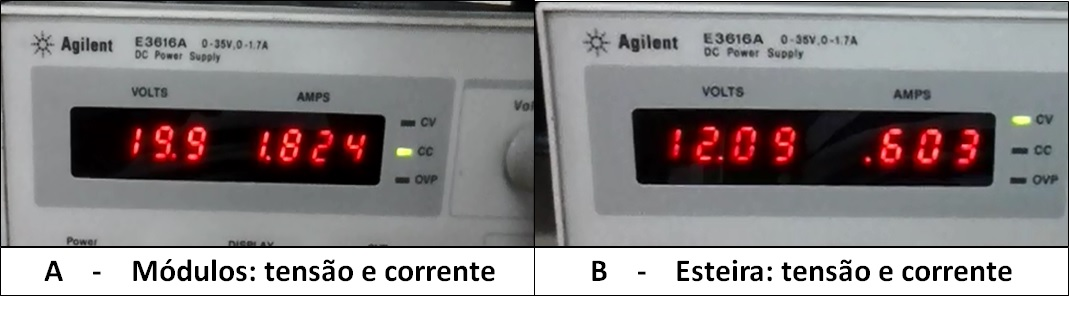
\includegraphics[width=12cm, height=3cm]{F126_SIAPE_TENSAO_CORRENTE.jpg} 
	\caption{SIAPE- Tensão e corrente}
	\label{F126}
\end{figure}

\subsection{Análise e validação dos requisitos RQ1 a RQ6}	

\begin{description}
	\item[Requisito RQ01 - Ciclo de produção:] O ciclo de produção é o tempo gasto nas atividades produtivas para produzir uma unidade de produto. Considerando a ilustração da Figura \ref{F120} o ciclo de produção é realizado entre os tempos t1 a t9, momentos em que a esteira e os atuadores são acionados pelo SIAPE. Nesse momento a esteira é parada e o módulo é acionado para carimbar o papel sobre o palete. O tempo de ciclo de um produto depende das quantidades de operações aplicados em sua produção, isto é o número de letras que são utilizadas para formar uma palavra. Assim para os produtos realizados na experimentação, foram registrados os seguintes tempos de ciclo:
		\begin{enumerate}
			\item Produto A = palavra UFAM: ciclo de 10,53 segundos
			\item Produto B = palavra UTAM:  ciclo de 10,63 segundos 
			\item Produto C = palavra UEA:  ciclo de 10,12 segundos
		\end{enumerate} 
		
	O Produto UFAM realizando os mesmos produtos obteve os seguintes ciclos de produção:
		\begin{enumerate}
			\item Produto A = palavra UFAM: ciclo de 15,42 segundos
			\item Produto B = palavra AFM:  ciclo de 10,55 segundos
			\item Produto C = palavra UTAM: ciclo de 15,33 segundos
		\end{enumerate} 
	
	\item[Requisito RQ02] - setup de produção é o tempo gasto com a configuração ou reconfiguração do sistema do produção. Na Figura \ref{F120}, o setup ocorre entre os tempos t1 e t2. Na experimentação foram produzidos três produtos e realizado dois setups de produção, no início do produto A e entre o produto B e C. Há que se enfatizar que o tempo de setup gasto entre os produtos B e C se deve à realização do conceito do plug and produce. Isso se deve à colaboração entre os agentes inteligentes que processam as alterações de produto e de quantidade entre os produtos A e B em tempo de processamento, não interferindo assim na produção. A Figura \ref{F125} ilustra o ganho reduzido de setup identificado no estudo de caso.
	
		\begin{figure}[h]
			\centering
			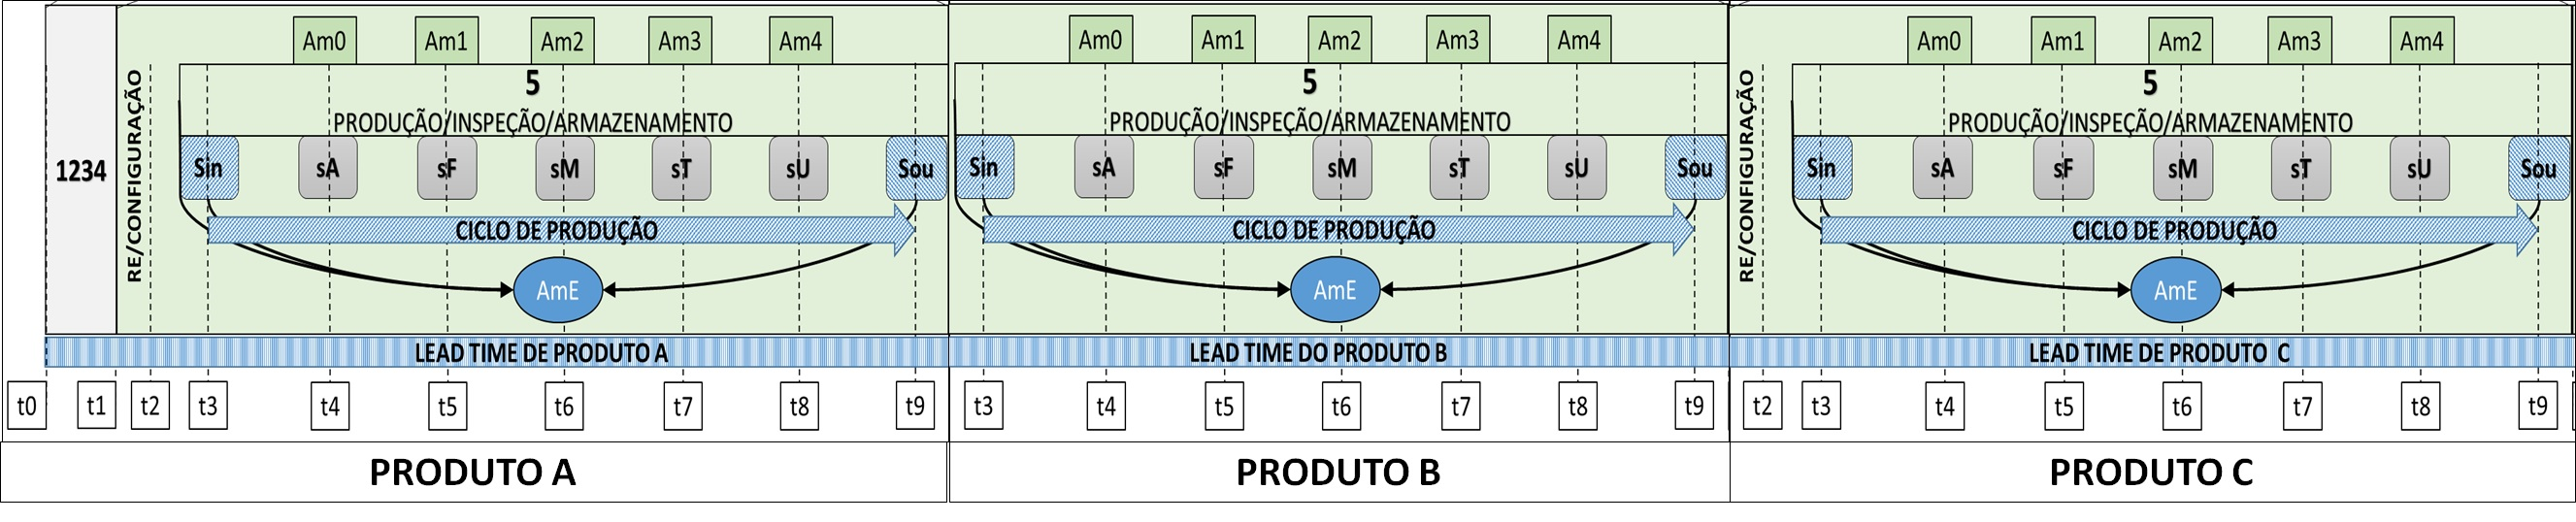
\includegraphics[width=16cm, height=5cm]{F125_SIAPE_CICLO_EXPLODIDOH.jpg} 
			\caption{SIAPE: Setup e Ramp up}
			\label{F125}
		\end{figure}	
	
	\item[Requisito RQ03] - ramp up de produção é o tempo gasto para que os recursos e operações na linha de produção sejam ajustados e se atinja a produção planejada. Na Figura \ref{F120} esse tempo encontra-se entre os tempos t10 e t11.  O SIAPE não gasta tempo com ramp up, pois os recursos do sistema são ajustados durante o tempo de setup para a produção planejada, não necessitando assim, do referido tempo. A eliminação de ramp up também está ilustrada na Figura \ref{F125}.
	
	
	\item[Requisito RQ04] -  Lead time de produto é considerado como o tempo gasto por todas as fases do ciclo de vida do produto  até que se produza uma unidade do produto da produção solicitada pelo cliente. Assim os tempos t0 a t11 cobrem o lead time de produto para este trabalho de pesquisa.  É importante notar que os tempos t11 a t12 cobrem um período em que não há mais desenvolvimento e os recursos e operações estão plenamente ajustadas.	
	
	
	\begin{figure}[h]
		\centering
		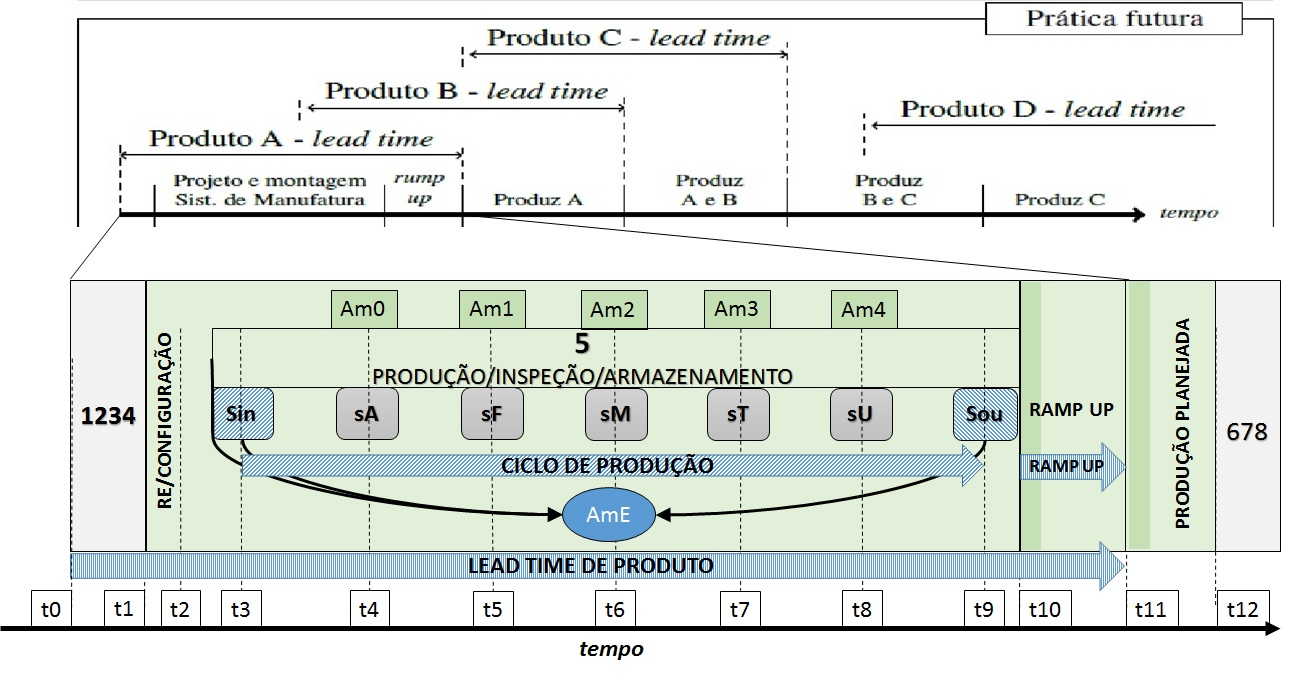
\includegraphics[width=16cm, height=10cm]{F120_2_SIAPE_CICLO_EXPLODIDO.jpg} 
		\caption{SIAPE: Lead time}
		\label{F120_1}
	\end{figure}	
	
	\item[Requisito RQ05] - O quinto requisito especificado pode ser evidenciado por meio da realização tanto do experimento quanto pelo exemplo ilustrado na Figura \ref{F123}.  Os módulos que carimbam as letras A, F, M, T e U foram desenvolvidos para atender esse requisito.\par 
	 
	\item[Requisito RQ06] - O sexto requisito especificado pelo cliente determina que palavras sejam originadas das letras disponíveis nos módulos. Mais uma vez é evidente o atendimento desse requisito pelo resultado do estudo de caso. A Figura \ref{F127} ilustra a identificação do módulo com relação à palavra onde o mesmo foi utilizado.


	\begin{figure}[h]
		\centering
		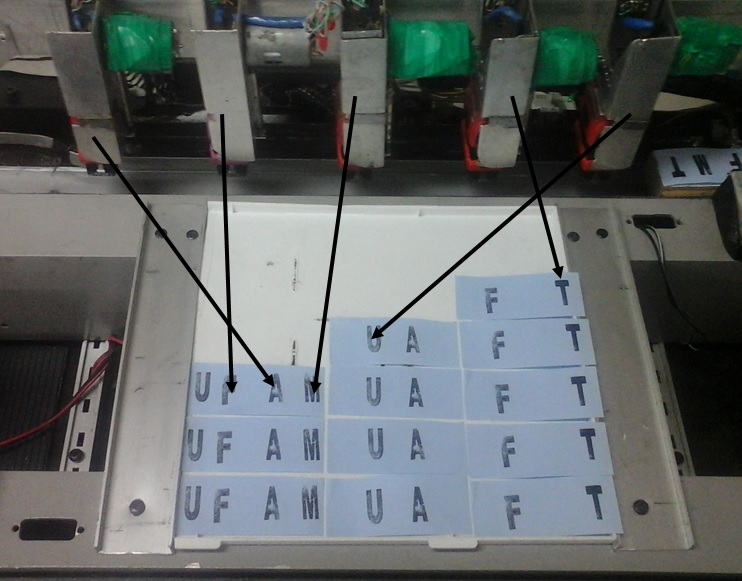
\includegraphics[width=14cm, height=5cm]{F127_SIAPE_AFMTU.jpg} 
		\caption{SIAPE: Anagramas, módulos e palavras}
		\label{F127}
	\end{figure}	


	
\end{description}					

\subsection{Análise e validação dos requisitos RQ07 a RQ12}	

\begin{description}
	\item[Requisito RQ07] - O requisito modularidade foi tratado desde a fase inicial do método de desenvolvimento MeDSE. Ao se refinar o problema global, em problema regional e depois em problema local tinha como principal objetivo refinar o problema até que ele chegasse ao nível atômico. Uma vez atingido esse nível, os problemas foram modelados, simulados especificados, implementados e validados modularmente, antes dos mesmos serem integrados e validados sistemicamente. É fácil perceber  por meio da verificação, primeiro, da Figura \ref{F13_1} na Fase de Realizações (etapas de 3 a 7) o desenvolvimento dos n módulos necessários para cada tipo de sistema. No caso do SIAPE, foram desenvolvidos cinco módulos para as letras A, F, M, T e U. Segundo, por meio da verificação das Figuras \ref{F69} e \ref{F70} o desenvolvimento dos módulos esteira e carimbador que realizaram a parte hardware do sistema, e na sequencia, a verificação das \ref{F71} a \ref{F74} e \ref{F94} o desenvolvimento dos módulos de software a partir das classes AcHw, YPA, Order, Anagrama e mensagens FIPA até que sejam simuladas. Nas Figuras \ref{F95} e \ref{F96} esses módulos são integrados às suas especificações que realizaram o projeto de sistema e o estudo de caso realiza a funcionalidade do sistema aplicado à produção de três produtos com qualidades e quantidades diferentes. 
	
	  
	\item[Requisito RQ08] - A plugabilidade no paradigma EPS é a propriedade que lida com a introdução de novos módulos, enquanto o sistema está em funcionamento. A eficiência do sistema nos tempos t4 a t8 é mantida por meio da reconfiguração dinâmica dos módulos, momento em que o sistema é rapidamente atualizado ao perceber que houve mudanças na disponibilidade de módulos no sistema. No estudo de caso a plugabilidade foi evidenciada na passagem da produção do produto B para o produto C, pois o módulo da letra T - realizou a palavra UTAM - foi conectado após a sua inclusão na interface gráfica. Essa propriedade é melhor detalhada durante a análise do processo que evidencia o conceito plug-and-produce (Plugar e produzir) explicado como uma das capacidades que  o SIAPE tem e que o permite adaptar-se e evoluir com o tempo.
		
	\item[Requisito RQ09] - Uma análise entre os produtos A e B percebe-se que existe uma diferença entre os anagramas UFAM e UTAM que é a letra T no lugar da letra F, implicando que o layout da linha deve ser alterado para que a produção dos anagramas sejam realizados. Contudo, a produção dos dois produtos foi realizada sem que houvesse qualquer interrupção na produção. Isso se deveu à reconfiguração do sistema originada pela negociação entre os agentes no mundo lógico -- conforme mostra a Figura~\ref{F144} -- que foi externada para o mundo real por meio do agente AcHw que atuou diretamente nos atuadores do hardware. Importante também perceber que a negociação foi realizada em paralelo à movimentação do produto A para o produto B, isto é, enquanto a esteira se movia no intervalo entre os produtos A e B, os agentes negociaram, e realizaram a negociação por meio das mensagens FIPA, e promoveram as mudanças necessárias à mudança de produto sem alterar a funcionalidade do sistema.	
	
		\begin{figure}[h]
			\centering
			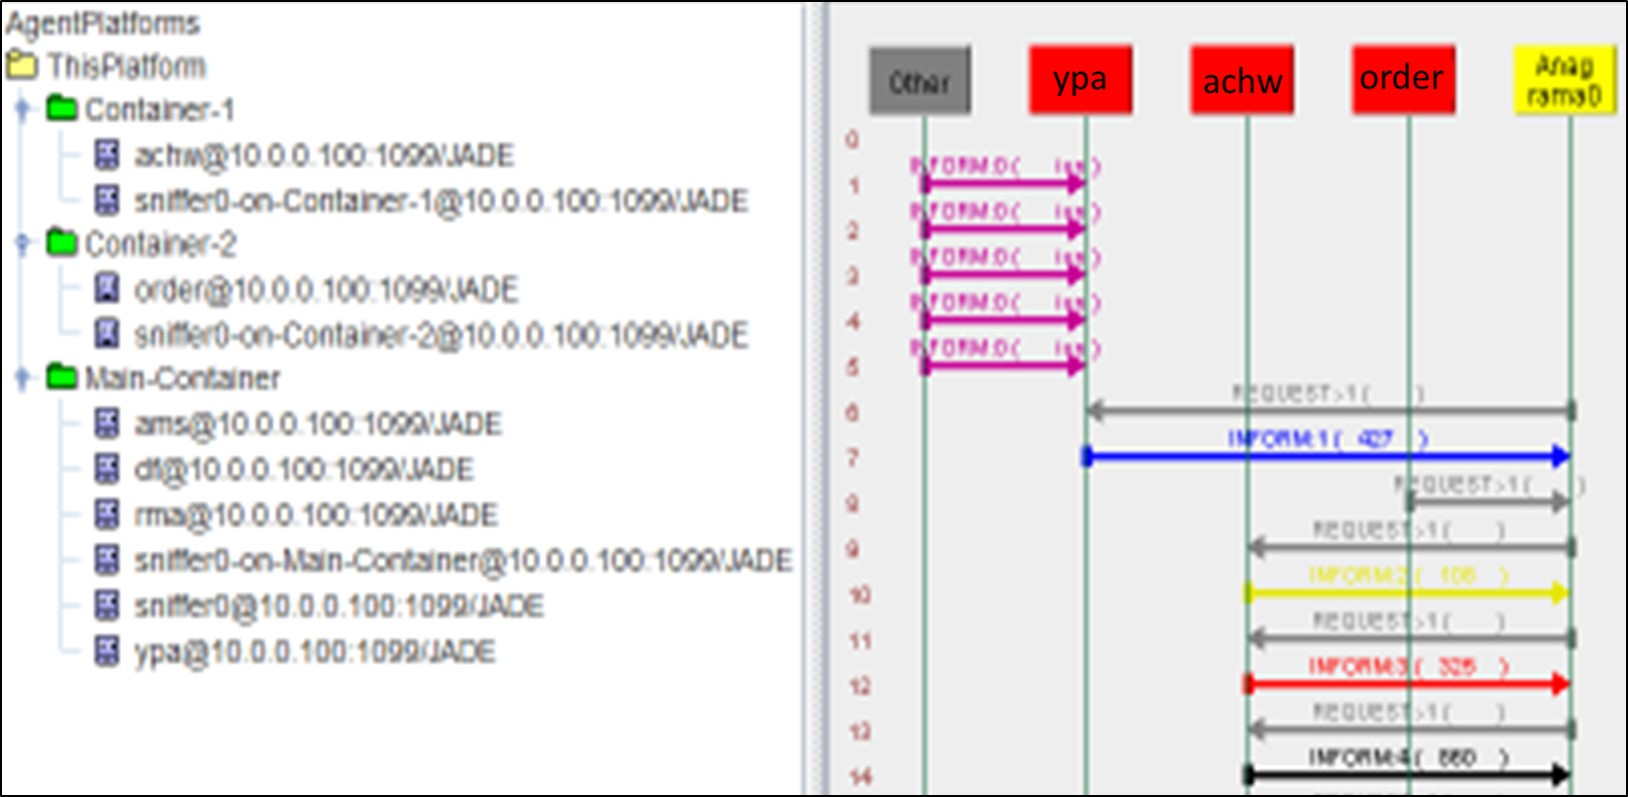
\includegraphics[width=14cm, height=5cm]{F144_ACL.jpg} 
			\caption{SIAPE: Negociação de agentes}
			\label{F144}
		\end{figure}	
		

	
	\item[Requisito RQ10] - A customização conforme definida neste trabalho é caracterizada por uma produção variada de produtos com curtos  ciclos de vida. Os lotes de produção são reduzidos para atender às solicitações personalizadas dos clientes. O experimento se enquadra nesse tipo de produção, pois realiza a produção de três produtos diferentes (UFAM, UTAM e UEA) com quantidades diferentes (3,4 e 5). A produção do produto A ocorre dentro dos padrões usuais atuais da indústria, contudo, na passagem do produto A para o produto B já percebe-se diferenças significativas na forma de produzir devido à ausência de reconfiguração e ramp up. Entre o produto e B e C, outra diferença é percebida por haver a inclusão de um módulo no sistema e o tempo gasto com essa operação durar menos de 20\% do tempo normalmente gasto nesse tipo e operação. Isso utilizando  sistema que não são baseados nos sistemas evolutivos, como o exemplo utilizado aqui denominado de Produto UFAM. \par 
	O tratamento realizado no estudo de caso evidencia um potencial promissor em tratar com a questão recorrente da customização de massa. É claro que tanto o tamanho da amostra quanto a própria forma do sistema aqui desenvolvido - em escala reduzida - e a forma e quantidade dos produtos, não favorecem análises mais acuradas, contudo da mesma forma é inegável que os dois sistemas tanto o produto UFAM baseado em ambientes 3.0 quanto o Produto SIAPE baseado no paradigma evolutivo, portanto em sistemas 4.0, são válidos por serem desenvolvidos por um método sistemático de desenvolvimento, o MeDSE, que possibilita a criação de sistemas que podem ser validados e realizados, a exemplo do SIAPE.
		
	\item[Requisito RQ11] - Este requisito foi solicitado para que se evidenciasse a presença do Governo influenciando no desenvolvimento e realização de sistemas de produção no território brasileiro. Assim foram incluídos circuitos que torna o sistema seguro baseado o nas normas NR-12 no item de Segurança no Trabalho em Máquinas e Equipamento que estabelece os procedimentos obrigatórios nos locais destinados a máquinas e equipamentos. Neste item estabelece que as máquinas devem ser equipadas com um ou mais dispositivos de parada de emergência, por meio dos quais possam ser evitadas situações de perigo latentes e existentes. As chaves podem cortar o processamento ao nível de software ou alimentações específicas a nível de hardware. \par 
	A exemplo no nível de hardware a Figura \ref{F128} ilustra alguns trechos de códigos e de partes do esquema elétrico do SIAPE para evidenciar  a atuação da chave SNR--12. A explicação dessa figura deve ser acompanhada com a visualização da Figura \ref{F123}. Na parte inferior (A) da Figura \ref{F128}  a linha de código evidenciada ilustra o comando que aciona a esteira. Quando a chave SRN$-12_1$ está fechada o exemplo ilustrado na Figura \ref{F123} funciona sem interrupção. Considere agora que na passagem do módulo M para o módulo U o operador necessite parar o processo. Ele aciona a chave colocando-a na posição aberta. Na parte de software a informação sai do Raspberry Pi (RPI) e polariza o fotoacoplador (U9) e este, chaveia o transistor Q1, contudo o relé RL1 não consegue ser acionado porque a alimentação de 24V foi interrompida pela RN--12. Quando o operador fechar novamente a chave, o sistema volta a funcionar normalmente e a letra U é carimbada. Isso se deve à linha de código na parte superior (A) da Figura \ref{F128} acionar o motor do módulo somente após a detecção do palete do módulo U (sU) nos limites do módulo U.\par 
	O exemplo demonstra um dos circuitos utilizados para evidenciar o atendimento desse requisito no experimento. 
	
	
		\begin{figure}[h]
			\centering
			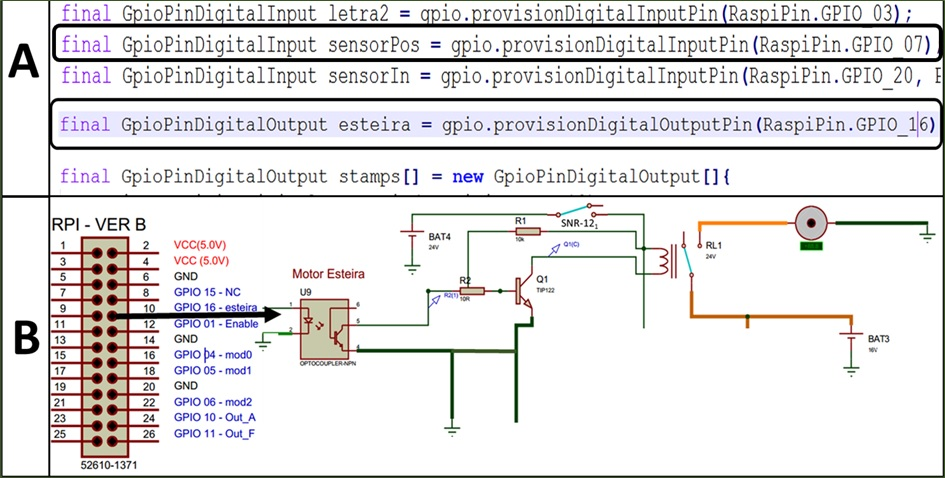
\includegraphics[width=14cm, height=7cm]{F128_SIAPE_SEGURANCA.jpg} 
			\caption{SIAPE: NR-12 Segurança}
			\label{F128}
		\end{figure}	
	
	\item[Requisito RQ12] - O requisito Custos nessa análise está relacionado à área da Economia para expressar a necessidade do cliente em ter os seus produtos competitivos no mercado local e global. Dois fatores são aqui considerados para que o produto seja competitivo: preço e entrega. Os ganhos de tempo nas operações de configuração e ramp up, levarão a reduções de tempo que implicarão na redução dos fatores de produção e o fato do sistema ser evolutivo o capacita a atender pequenas quantidades de produtos e consequentemente, aumentando a competitividade dos produtos produzidos por esse produtor. A agilidade dos sistemas evolutivos em responder às mudanças da demanda não afetam a produção aos níveis praticados hoje por sistemas de ambientes 3.0.
	
\end{description}	

\subsection{Análise e validação dos requisitos RQ13 a RQ15}	
				
\begin{description}
	\item[Requisito RQ13] - Os primeiros trabalhos de Especificação para a arquitetura da Internet das Coisas \textit{(IoT)} procurou evidenciar especificamente a atualização do estado da arte para questões relacionadas com a Plug \& Play, a partir de um ponto de vista de Internet de Coisas, na fabricação e automação, bem como na aquisição de requisitos funcionais. Essa primeira iteração teve o objetivo de coletar os aspectos mais centrais e críticos de Plug \& Work (Plugar e trabalhar) no ambiente industrial, isto é, num sistema em funcionamento, pode-se incluir um módulo do sistema e esse iniciar imediatamente o seu funcionamento sem causar a necessidade de parar o sistema para realizar essa operação. \par 
	
	A análise relatada  no documento identificou três cenários principais diferentes. Aqui neste trabalho considerou-se especificamente as questões relacionadas no Apêndice B que trata a manufatura ágil. Como Manufatura Ágil o apêndice define uma produção fortemente baseada na disponibilidade da tecnologia de fabricação que pode ser facilmente reconfigurada para responder rapidamente às contínuas mudanças do mercado e continua a fornecer controle total da produção custos e qualidade. \par 
	Como pode ser entendido pela redação o conceito de \textit{plug-and-produce} vai além do conceito de \textit{plug \& work} pois além de plugar e produzir, \textit{plug-and-produce} prevê tanto a inclusão quanto  exclusão de um módulo no sistema sem reduzir a performance do mesmo. Esse conceito foi evidenciado na passagem do produto B para o produto C.	
	
	\item[Requisito RQ14] - A Indústria 4.0 é um conceito que se transforma em realidade com a realização de mudanças no mundo da produção industrial. O aumento exponencial da capacidade dos computadores possibilita a realização de muitos algoritmos até então não realizados pela capacidade das máquinas, a grande quantidade de informação digitalizada e as novas estratégias inovadoras de pessoas, pesquisas e tecnologia concretizam rapidamente esse novo ambiente no globo terrestre.\par 	
Uma empresa com características da Indústria 4.0 dispõe em sua planta fabril de dispositivos que são reconhecidos de duas formas: A primeira forma por sua estrutura física por meio das máquinas equipamentos e recursos utilizados no mundo real. A outra forma é por sua estrutura virtual, ou seja,  por seus IDs ao entrarem no domínio de uma rede de comunicação. Esses dispositivos uma vez reconhecidos, podem ser configurados e utilizados em sistemas evolutivos com níveis elevados de flexibilidade, plugabilidade, modularidade, escalabilidade, interoperabilidade, agilidade, auto-organização, precisão e outras propriedades comuns aos dispositivos que sofreram a influência da 4a Revolução Industrial. Uma planta formada por módulos mecatrônicos, por dispositivos eletromecânicos, mecânicos e eletrônicos comandados por sistemas de computação baseados em paradigmas de multi-agentes inteligentes pode desempenhar atividades que denotam a inteligência necessária e suficiente para atender às alterações de demanda de produtos dentro de um sistema de manufatura. Somando-se ao atendimento da demanda, o fato da redução de setup a nível que tendem a zero, através da modularidade das partes do sistema, consegue-se a escalabilidade a níveis que atendam a urgência de produção da Customização e tem-se a concretização de sistemas evolutivos como potencial solução do problema de lotes pequenos que tem inviabilizado os atuais sistemas de produção. \par

Num futuro próximo, a instalação de produção reconhecerá por si própria (a esteira e o palete codificado acionado pelo agente AcHw) o que terá de fazer em cada nova peça ou produto. A forma de codificação utilizada poderá variar de acordo com o avanço da tecnologia, no SIAPE a codificação utilizada foi a marcação lateral com hastes metálicas que são detectadas por sensores magnéticos (sA, sF, sM, sT e sU) mas poderia ser na forma de um chip eletrônico, uma identificação para leitura RFID ou até mesmo código de barras. Cada vez mais o produto será fabricado de acordo com os desejos individuais do cliente.

Em outras palavras isto quer dizer, para cada objeto real tem de haver uma imagem virtual para que possa comunicar-se posteriormente com outras máquinas ou peças. As partes real e virtual poderão comunicar-se apenas no nível virtual. No nível virtual são realizadas as operações complexas e tomadas as decisões que demandem inteligência e raciocínio. O resultado é comunicado à parte real que realiza a decisão correta a ser realizada, por exemplo, a produção do estudo de caso. A expansão do mundo virtual cria a possibilidade de comunicação com outras máquinas e sistemas que realizam finalmente o conceito da integração Horizontal recomendada pela Plataforma da Indústria 4.0.
	
	\item[Requisito RQ15] - O estado da arte originado da relação com a Academia foi incluído como forma de evidenciar que os sistemas evolutivos, baseados no paradigma evolutivo é na atualidade, o que existe de mais promissor como solução para o problema da indústria que trata da customização de massa.
	
A Academia em todo o mundo faz as pesquisas na busca da realização da Indústria 4.0 que requer respostas e soluções para diferentes tópicos como cyber-segurança, padrões aceitáveis e interoperabilidade entre máquinas e sistemas, e sustentabilidade. 
		
\end{description}	

%==========================================VALIDAÇÃO==========================================

\newpage


\subsection{Comparações SIAPE versus Produto UFAM}

%
% 	 \subsection{Descrições: Arquitetura IADE, implementações de Cavalcante, e de Rosa}
% 	 
% 	 Dentre os diversos programas desenvolvidos pela União Europeia (UE) o Programa Quadro 7 (FP7) tratou de questões ligadas à investigação e Desenvolvimento Tecnológico. Foi o principal instrumento da UE para financiar a investigação na Europa e fora dela, e esteve em vigor de 2007 a 2013. Esse programa nasceu da necessidade de se criar mais empregos europeus e aumentar a competitividade da UE. O FP7 era formado por cinco programas específicos: 1) Programa Cooperação na investigação colaborativa 2) Programa IDEAS: Conselho Europeu de Investigação que concentrou-se em investigação de ponta; 3) Programa Pessoas que objetiva o potencial; 4) Programa Capacidades que trata de pesquisa na União Europeia e o 5) Programa Nuclear que trata da investigação e formação na área de energia nuclear. Dentre esses projetos, em especial, o Projeto \textit{IDEAS}~\cite{ONORI2012} serviu como prova de conceitos para os Sistemas Evolutivos baseados no paradigma EPS. \par 
% 	 
% 	 A Universidade Federal do Rio Grande Sul participou do IADE com alunos de Doutorado, e dentre os trabalhos resultantes foi apresentada a  Tese de Doutorado que contribuiu com a Arquitetura Baseada em Agentes e Auto-Organizável Para a Manufatura ~\cite{CAVALCANTE2012} que introduziu os conceitos de Sistemas Evolutivos Aplicados à Manufatura, no Brasil. %e 2) O Desenvolvimento de Sistemas de Automação da Manufatura Usando Arquiteturas Orientadas a Serviços e Sistemas Multi-agentes  \cite{PEIXOTO2012}. \par 
% 	 
% 	 Em 2013 Rosa  contribuiu para o  projeto de IDEAS  aumentando a consciência de que a auto-organização de sistemas mecatrônico não são, necessariamente imprevisível, quando a dinâmica desses sistemas pode ser explicada. Rosa estudou as interações entre alguns dos agentes, os simulou, para descobrir a dinâmica oculta da auto-organização no contexto do projeto IDEAS, e elabarou uma métrica de decisão que foi aplicada ao sistema a fim de quantificar a probabilidade de alguns agentes tomarem algumas decisões durante o processo de produção. \par 
% 	 
%	
%	%===============================================IADE====================================================
%	
%		\subsection{Descrição do IADE}
%		
%	Esta subseção tem como meta avaliar, primeiramente, a implementação de hardware do SIAPE com o Produto UFAM e no segundo momento validar a implementação de software do SIAPE com os resultados que validaram as arquiteturas de Cavalcante e Rosa no ambiente IDEAS e mostrar que a implementação de software do SIAPE operando com o hardware baseado no Produto UFAM é conceitual e empiricamente válido.  
%	
%	O IDEAS Agent Development Environment (IADE) é uma biblioteca desenvolvida dentro dos limites do projeto IDEAS. A arquitetura IADE é aderente à infra-estrutura de agente de JADE \cite{WOOLDRIDGE2007}  que suporta o protocolo de comunicação FIPA \cite{FIPA2013}. Por sua vez, o projeto Instantly Deployable Evolvable Assembly Systems (IDEAS) foi o primeiro hardware que realizou os estudos iniciais do IADE e era dotado, conforme 	\cite{RIBEIRO2011}, dos quatro agentes básicos identificados na Figura \ref{F139} que são descritos a seguir:\par 
%
%		\begin{description}	
%			
%			\item [1 - Máquina Resource Agent (MRA)] - A MRA é responsável pelo controle de módulos que podem ser conectado e desconectado diretamente no sistema. ;
%			\item [2 - Coalition Líder Agent (CLA)] - O CLA permite que a composição de skills seja executada. O CLA apoia a lógica de execução de processos que são projetados pelo usuário com base nos skills disponíveis no sistema; 
%			\item [3 - Agente Transporte de sistema ou Agent Unidade de Transporte (TSA / TUA)] - esses componentes resumem o sistema de transporte TSA. Ele fornece a localização, funcionalidades de transporte e posicionamento. Cada TSA mantém pista da sua própria posição no sistema, que é tipicamente associado com a posição de um MRA ou CLA no sistema.	
%			\item [4 - Agente para Machine Interface ( AMI )] - O trabalho do agente AMI é funcionar como uma camada de harmonização entre as configurações de hardware dedicado e os MAs. 			
%		\end{description}	
%
%	Conforme Ribeiro, estas quatro classes de agentes encerram e abstraem toda a interação genérica entre as entidades do chão de fábrica. No entanto, eles podem ser estendido para incorporar detalhes sobre equipamentos específicos sem alterar  os padrões de interação entre agentes. Os pesquisadores, neste caso Cavalcante e Rosa, estenderam essas classes ao demonstraram as características do paradigma evolutivo, isto é, realizaram o conceito plugar-e-produzir que capacitou os sistemas industriais a adaptar-se e evoluírem.
%	
%		 \begin{figure}[h]
%		 	\centering
%		 	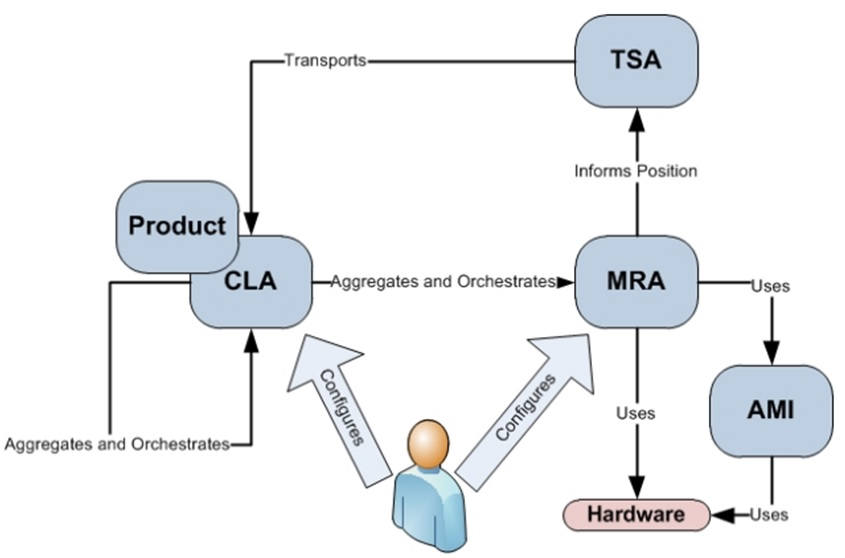
\includegraphics[width=12cm, height=6cm]{F139_IDEAS.jpg} 
%		 	\caption{IDEAS Mechatronic Multiagent Architecture (IMMA)}
%		 	\footnotesize{Fonte: \cite{RIBEIRO2011}}
%		 	\label{F139}
%		 \end{figure}
%	
%	Os trabalhos validados no ambiente IADE foram validados em período de tempo diferentes. Cavalcante realizou sua arquitetura em 2012 com utilização dos seguintes hardware no ambiente IADE: Célula Festo, Pré-demonsttrador IDEAS e numa simulação de esteira. Em 2013, o ambiente IADE foi finalizado e acrescido do hadware MASMEC, uma integração de todos os dispositivos ne mesma planta, e Rosa validou sua arquitetura com os seguintes hardwares: Célula Festo, Pré-demonsttrador IDEAS e Demonstrador MASMEC. O SIAPE foi comparado com os resultados no Pré-demonstrador IDEAS que foi utilizado na validação de ambas as arquiteturas. \par 
%	
%	A Figura \ref{F136} ilustra a planta do Pré-demonstrador IDEAS. Na parte (a) o registro de um instantâneo do IADE  em funcionamento, na parte (b) a ilustração do layout  do IADE na visão de Cavalcante, e na parte (c) o layout na visão de Rosa. \par 
%		
%	 \begin{figure}[h]
%	 	\centering
%	 	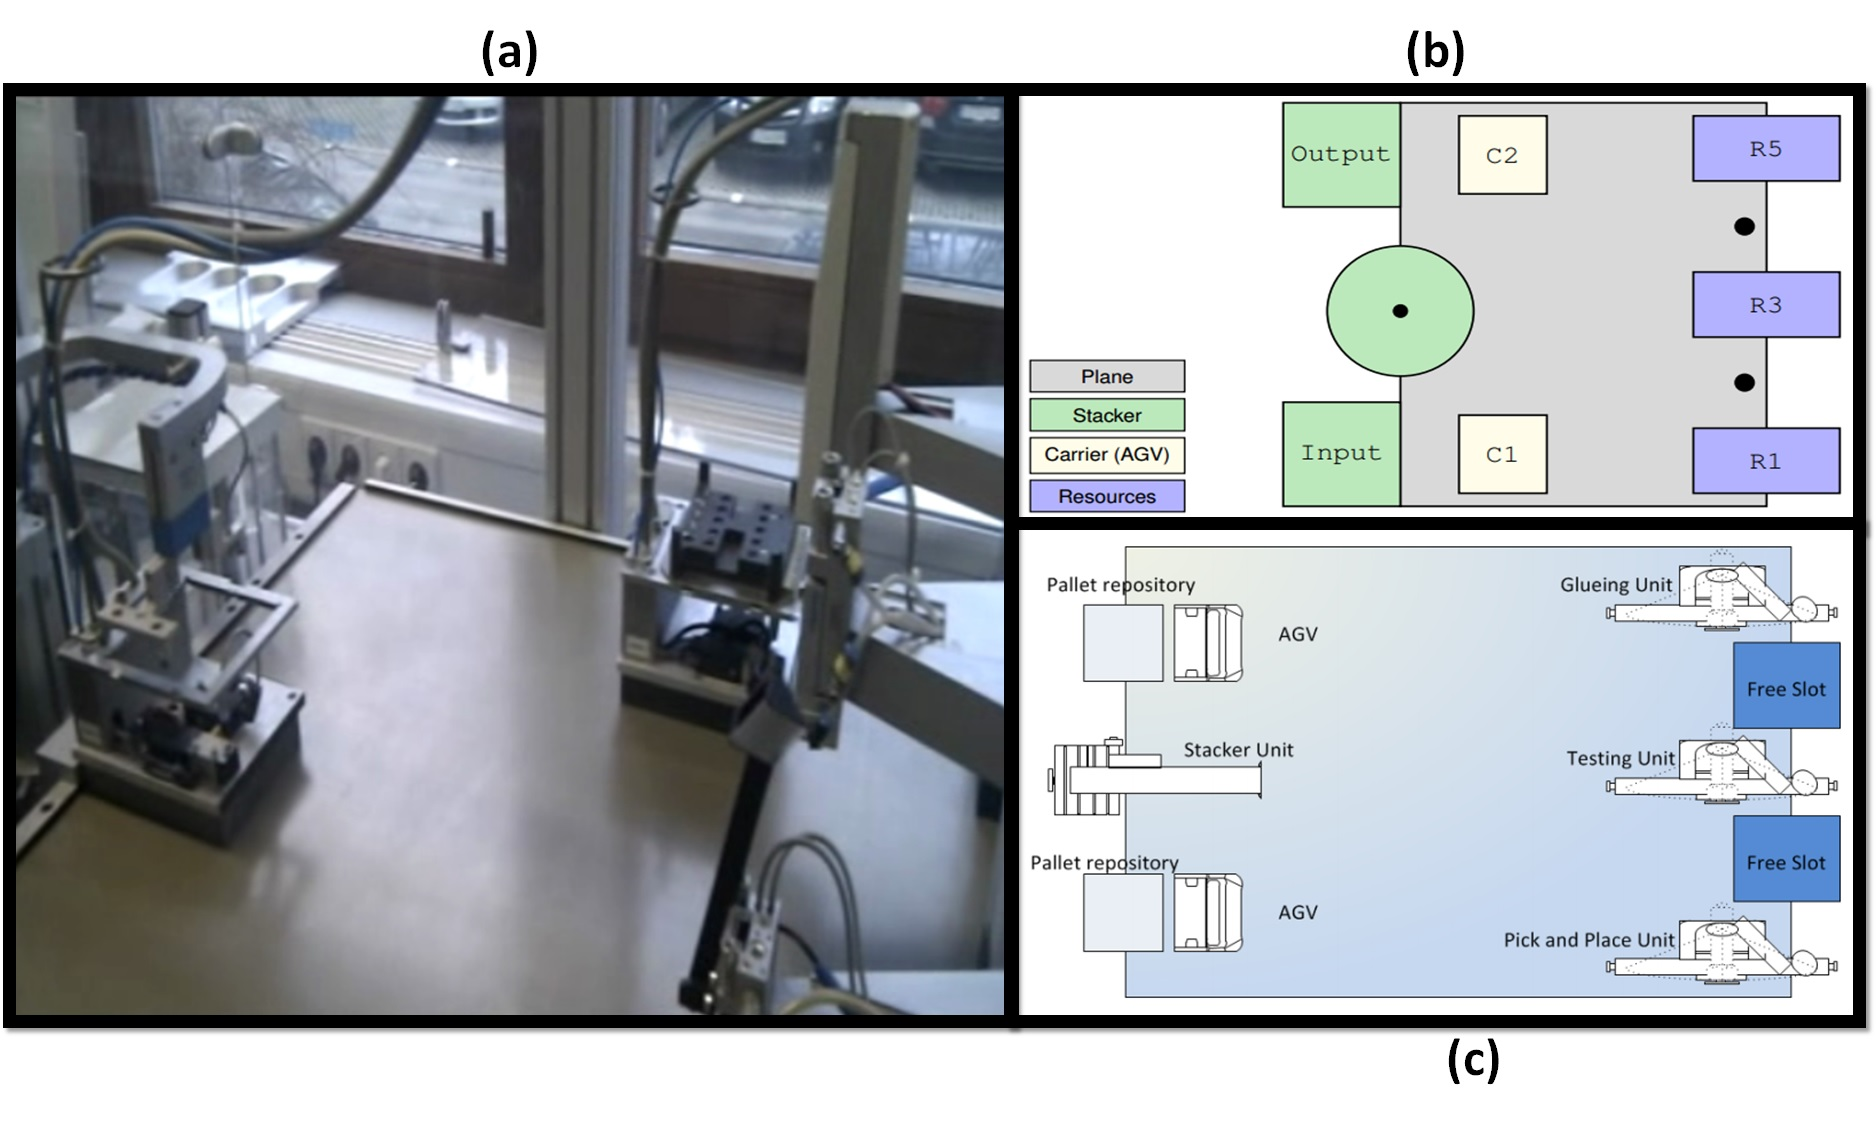
\includegraphics[width=16cm, height=10cm]{F136_IADE_CAVALCANTE_ROSA.jpg} 
%	 	\caption{IADE: Layout por Cavalcante e Rosa}
%	 	\footnotesize{Fonte: \cite{CAVALCANTE2012} \cite{ROSA2013c}}
%	 	\label{F136}
%	 \end{figure}
%
%	Para explicar o funcionamento utilizou-se uma ilustração de Rosa que mostra o funcionamento básico do Pré-demonstrador IDEAS e está reproduzido na Figura \ref{F137} onde o funcionamento é explicado pelo autor com a utilização das três possíveis posições horizontais básicas do eixo empilhador do IDEAS: \par
%		
%	\begin{description}	
%	
%\item [1 - Na posição (a) da Figura \ref{F137}], a empilhadora está posicionado para pegar um palete do carro AGV, ou colocar o palete no carro AGV;
%\item [2 - Na posição (b) da Figura \ref{F137}] está ilustrada a operação para recuperar o palete no repositório de entrada; 
%\item [3 - Na posição (c) da Figura \ref{F137}] finalmente, a empilhadora deve ser posicionado para armazenar um palete para o repositório de saída, .
%
%	\end{description}		
%	
%As possíveis posições horizontais do Pré-demonstrador IDEAS foram implementadas para realizar cada arquitetura de cada pesquisador. \par As implementações para validar as arquiteturas são discutidas a seguir.
%
% \begin{figure}[h]
% 	\centering
% 	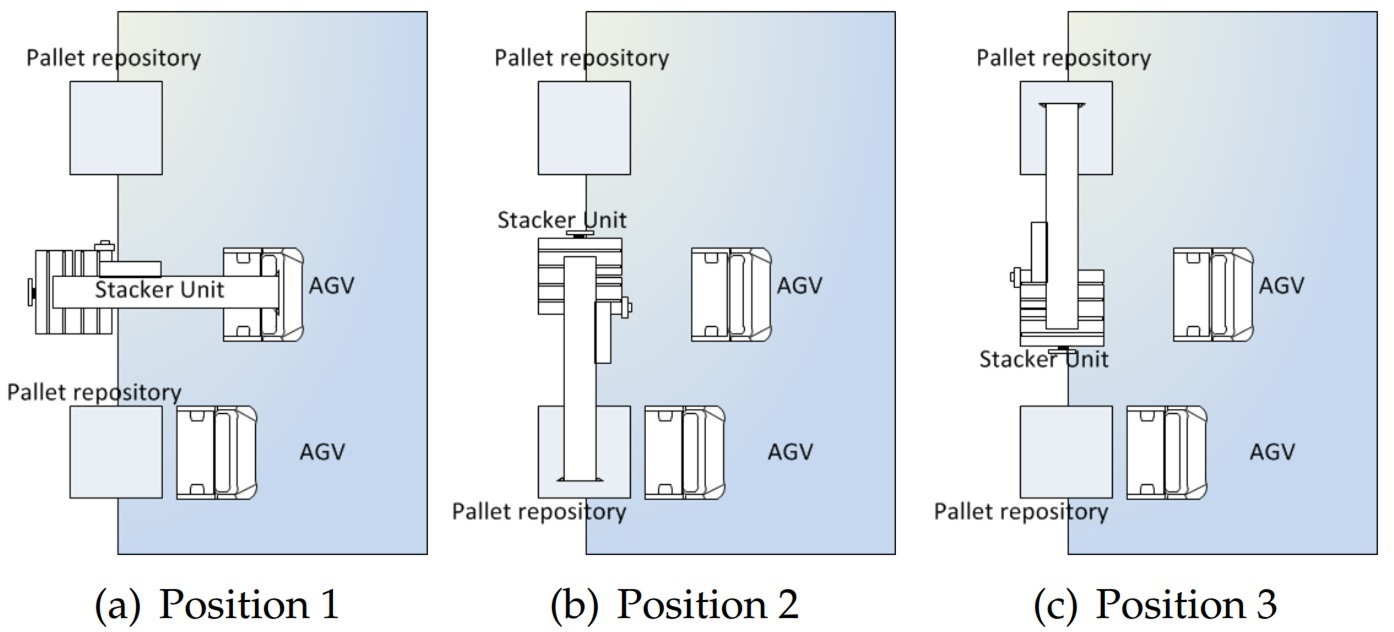
\includegraphics[width=16cm, height=5cm]{F137_IADE_3POSICOES_ROSA.jpg} 
% 	\caption{IADE: Explicação funcionamento IDEAS por Rosa}
% 	\footnotesize{Fonte: \cite{ROSA2013c}}
% 	\label{F137}
% \end{figure}
%		
%========================================================================================


%Esta subseção compara os desempenhos encontrados entre o SIAPE e o Produto UFAM. 

O plano de produção realizado na experimentação foi expandido para uma quantidade de 10 unidades de produtos. Os tempos decorridos na produção estão registrados na Tabela~\ref{T16}. Todos os tempos em segundos \textbf{(s)}. O tempo médio de palavras com quatro letras realizadas no SIAPE (por exemplo UFAM e UTAM) foi de 10 segundos enquanto a mesma produção realizada no Produto UFAM apresentou uma média de 15 segundos. Para palavras com três letras o SIAPE registrou o tempo de respectivamente de 9 e 10 segundos. O incremento representa um aumento no tempo decorrido de 32\% a mais no Produto UFAM para realizar a mesma produção realizada no SIAPE.

\begin{table}
	\small
	\centering
	\caption{SIAPE X PRODUTO UFAM: TEMPO DE PRODUÇÃO (s)}
	\begin{tabular}{ c | c c | c c | c c }
		\hline
\textbf{ Palavra} & \multicolumn{2}{c}{\textbf{UFAM}}  & \multicolumn{2}{c}{\textbf{UTAM}} & \textbf{ UEA} & \textbf{ AFM} \\ \hline
\textbf{Item} & \textbf{SIAPE} & \textbf{PUFAM} & \textbf{ SIAPE} & \textbf{ PUFAM} & \textbf{ SIAPE} & \textbf{ PUFAM}\\ 
		\hline
 
  01 & 10,16 &  14,70  & 10,66 & 15,70 & 10,20 &  10,67 \\ \hline
  02 & 10,17 &  16,68  & 10,71 & 14,66 & 9,92  &  10,44 \\ \hline
  03 & 10,88 &  15,59  & 10,49 & 16,50 & 10,30 &  10,56	\\ \hline
  04 & 10,07 &  15,55  & 10,57 & 15,03 & 10,20 &  10,67	\\ \hline
  05 & 10,04 &  15,60  & 10,64 & 15,55 & 10,10 &  10,66	\\ \hline
  06 & 10,72 &  15,60  & 10,72 & 15,04 & 10,10 &  10,45	\\ \hline
  07 & 10,72 &  15,55  & 10,72 & 15,58 & 10,19 &  10,34	\\ \hline
  08 & 10,94 &  14,90  & 10,44 & 14,97 & 15,10 &  10,45	\\ \hline
  09 & 10,91 &  14,94  & 10,71 & 14,95 & 10,20 &  10,67 \\ \hline
  10 & 10,73 &  15,11  & 10,73 & 15,30 & 10,10 &  10,56	\\ \hline
  \hline
  Média & 10,50 &  15,42 	& 10,60 & 15,33 & 9,10 &  10,55	\\ \hline
 	\end{tabular}												
	\label{T16}\par
	%	Fonte: Hiram Amaral
\end{table}

Existem alguns motivos que explicam essa vantagem no desempenho do SIAPE em relação ao Produto UFAM. Dois desses motivos estão registrados na Tabela \ref{T17} e são explicados na sequência. \par 

Na segunda coluna da Tabela \ref{T17} estão registrados os dados coletados no SIAPE quando o agente Stamper realiza seu skill carimbar letra. O tempo médio da realização deste skill é de 1 segundo contra 3 segundos registrados na operação das válvulas pneumáticas do Produto UFAM. A diferença em torno de 2 segundos é explicada pelo fato do circuito elétrico do motor DC, utilizado nos módulos do SIAPE, reagir com maior eficácia  quando comparado ao circuito eletro-pneumático do Produto UFAM, pois o circuito só reage, primeiramente com os solenóides, e depois os solenóides liberam as válvulas pneumáticas que realizam a operação carimbar letra. Esses tempos reduzem o desempenho do produto UFAM para esse nível de produção nas condições aqui consideradas.\par

Outro motivo que reduz também o desempenho do Produto UFAM para as condições apresentadas é o fato do sistema ter sido projetado para que o operador aguarde a finalização do produção de um produto e reinsira o palete na entrada do sistema. Essa operação registrou um tempo médio de 3 segundos contra 1 segundo do SIAPE. No SIAPE os paletes já encontram-se agregados à esteira, cabendo ao operador apenas retirar os produtos realizados. 

As colunas 6 e 7 da Tabela \ref{T17} registra os tempos com a troca de módulos com o SIAPE em funcionamento. O tempo médio para realizar a troca de um módulo pelo operador, com a detecção deste pelo agente AcHw e posterior inclusão do novo recurso no plano de produção alcançou a média de 45 segundos. Vale registrar que esse tempo iniciou-se em torno de 4 minutos que foi reduzido para 2 minutos até alcançar o tempo atual registrado. Apesar do tempo reduzido este processo que realiza o \textit{plug and produce} pode ser reduzido ainda mais por meio de melhorias no hardware.  A sétima coluna registra o fato dessa mesma operação ser realizada no Produto UFAM, dado que os procedimentos exigiriam a parada do sistema elétrico e do sistema pneumático para posterior troca mecânica da válvula pneumática.

\begin{table}[!h]
	\centering
	\caption{SIAPE X PRODUTO UFAM: STAMPER, OPERADOR e TROCA(s)}
	\footnotesize
	\begin{tabular}{C{1cm} | C{1.5cm} C{1.5cm} | C{1.7cm} C{1.7cm} | C{1.2cm} C{1.5cm}} 
		\hline
	    \textbf{Item} & \textbf{SIAPE Stamper} & \textbf{PUFAM Stamper} & 
        \textbf{SIAPE Operador} & \textbf{PUFAM Operador} & \textbf{SIAPE Troca} & \textbf{PUFAM Troca} \\

		\hline
		\hline
		  01  & 1,79 & 3,30 & 1,89 & 3,06 & 48,73 &  \multirow{11}{*}{\begin{sideways}I m p r a t i c á v e l\end{sideways}} \\ \cline{1-6}
		  02  & 1,87 & 2,86 & 1,89 & 2,83 & 46,25 &  \\ \cline{1-6}
		  03  & 1,64 & 3,50 & 1,86 & 3,20 & 49,25 &  \\ \cline{1-6}
		  04  & 1,72 & 4,19 & 1,62 & 3,39 & 50,25 &  \\ \cline{1-6}
		  05  & 1,88 & 3,42 & 1,95 & 3,50 & 42,65 &  \\ \cline{1-6}
		  06  & 1,76 & 3,50 & 1,98 & 4,01 & 43,25 &  \\ \cline{1-6}
		  07  & 1,67 & 3,51 & 1,87 & 3,09 & 44,50 &  \\ \cline{1-6}
		  08  & 1,54 & 3,80 & 1,89 & 3,55 & 46,20 &  \\ \cline{1-6}
		  09  & 1,67 & 3,86 & 1,87 & 2,86 & 43,25 &  \\ \cline{1-6}
		  10  & 1,88 & 3,64 & 1,88 & 3,22 & 44,30 &  \\ \cline{1-6}
		  \hhline{======}
		Média & 1,74 & 3,56 & 1,90 & 3,27 & 45,86 &  \\ \hline
		
	\end{tabular}												
	\label{T17}\par
	%	Fonte: Hiram Amaral
\end{table}

A Tabela \ref{T18} registra o melhor desempenho do Produto UFAM no trato do \textit{bootstrap} do sistema. Conforme explicado no Capítulo 4 o ambiente deve ser configurado seguindo os procedimentos relacionados nos itens de 1 a 6 e que foram ilustração na Figura \ref{F105}. Essa configuração foi registrada no SIAPE com uma média de 2,5 minutos contra os 9 segundos do Produto UFAM.  Vale lembrar que essa configuração é feita apenas uma vez durante um dia de produção. 

\begin{table}[!h]
	\centering
	\caption{SIAPE X PRODUTO UFAM: TEMPO DE BOOTSTRAP (s)}
	\begin{tabular}{c | c  c } \hline
		\multirow{2}{*}{Item} & \multicolumn{2}{c}{\textbf{BOOTSTRAP}} \\ \cline{2-3}
								  & \textbf{SIAPE} & \textbf{PUFAM}       \\ \hline
		\hline
		01 & 150 &  \textbf{9,53}  \\ \hline
		02 & 150 &  \textbf{9,63}  \\ \hline
		03 & 150 &  \textbf{9,50}  \\ \hline
		04 & 150 &  \textbf{9,39}  \\ \hline
		05 & 150 &  \textbf{9,36}  \\ \hline
		06 & 150 &  \textbf{9,39}  \\ \hline
		07 & 150 &  \textbf{9,36}  \\ \hline
		08 & 150 &  \textbf{9,36}  \\ \hline
		09 & 150 &  \textbf{9,39}  \\ \hline
		10 & 150 &  \textbf{9,36}  \\ \hline
		\hline
			             
		Média & 150 & \textbf{9,43}  \\ \hline
		
	\end{tabular}												
	\label{T18}\par
	%	Fonte: Hiram Amaral
\end{table}
 	
A Tabela \ref{T19} registra os tempos médios totais dos produtos realizados no plano de produção durante a experimentação realizada que foi descrita no Capítulo 4. Esses tempos foram medidos de acordo com os parâmetros definidos na primeira subseção deste capítulo e a Figura \ref{F123} auxilia no entendimento da discussão. \par 

Nas colunas 2 e 3 estão identificados os tempos totais gastos (montante e percentual) nos lotes dos produtos A, B e C durante a experimentação. Os dados registrados são importantes para evidenciar os desempenhos de ambos os sistemas de acordo com a situação desejada : \par 

\begin{description}
	\item[Produto A] O tempo total gasto na produção de 3 produtos do tipo A foi registrado com 46 segundos no Produto UFAM e 31 segundos no SIAPE, representando uma diferença de 33\% do tempo gasto a mais pelo Produto UFAM comparado ao desempenho do  SIAPE. Esse valor representa um tempo de 15 segundos gastos pelo Produto UFAM contra 10 segundos gastos pelo SIAPE para produzir uma unidade do produto A. Esses tempos evidenciam que os módulos realizam operações na faixa de 5 segundos no Produto UFAM e 3 segundos no SIAPE. 	
	
	\item[Produto B] O tempo total gasto na produção de 4 produtos do tipo B foi registrado com 61 segundos no Produto UFAM e 42 segundos no SIAPE, representando uma diferença de 31\% do tempo gasto a mais pelo Produto UFAM comparado ao desempenho do  SIAPE. Esse valor ainda representa um tempo de 15 segundos gastos pelo Produto UFAM contra 10 segundos gastos pelo SIAPE para produzir uma unidade do produto B. Esses tempos evidenciam que os módulos realizam operações na faixa de 3 segundos no Produto UFAM e 2 segundos no SIAPE. 	
		
	\item[Produto C] O tempo total gasto na produção de 5 produtos do tipo C foi registrado com 53  segundos no Produto UFAM e 50 segundos no SIAPE, representando uma diferença de apenas 4\% do tempo gasto a mais pelo Produto UFAM comparado ao desempenho do  SIAPE. Esse valor representa um tempo de 10 segundos gastos pelo Produto UFAM contra 10 segundos gastos pelo SIAPE para produzir uma unidade do produto B. Esses tempos evidenciam que os módulos realizam operações na faixa de 2 segundos tanto para o Produto UFAM quanto para o SIAPE. 
		
\end{description} 	 	 
 
\begin{table}
 	\small
 	\centering
 	\caption{SIAPE X PRODUTO UFAM: TEMPO DE PRODUÇÃO(s)}
 	\begin{tabular}{c c | c c | c c | c c | c}
		\multicolumn{2}{c|}{\textbf{Item}} & 
		\textbf{PUFAM} & \textbf{SIAPE} & 
		\textbf{PUFAM} & \textbf{SIAPE} & 
		\textbf{PUFAM} & \textbf{SIAPE} &
		\multirow{2}{*}{$\Delta\%$} \\
		
		\textbf{PROD} & \textbf{QTD} & 
		\multicolumn{2}{c|}{\textbf{t\underline{ }TOTAL}} &
		\multicolumn{2}{c|}{\textbf{t\underline{ }CICLO\underline{ }P}} &
		\multicolumn{2}{c|}{\textbf{t\underline{ }CICLO\underline{ }O}} &
		~ \\ \hline \hline
		
	 	A &  3  & 46,97 & 31,21  & 15,657 & 10,403 &  5,219  &  3,468 & 33,55 \\
	 	\hline
	 	
	 	B &  4  & 61,89 & 42,43  & 15,473 & 10,608 &  3,860  &  2,652 & 31,44 \\
	 	\hline
	 	
	 	C &  5  & 53,00 & 50,65  & 10,600 & 10,130 &  2,120  &  2,026 &  4,43 \\
		
		
	\end{tabular}
	\label{T19}\par
 	%	Fonte: Hiram Amaral
\end{table}

A análise da Tabela \ref{T19} evidencia que o aumento de lotes  de produção têm vantagens consideráveis para serem realizadas no Produto UFAM. Isso se deve ao fato do produto UFAM não utilizar uma plataforma de agentes inteligentes como ocorre com o SIAPE. Não utilizando agentes, não há necessidade do uso de protocolos de comunicação FIPA. Não havendo comunicação, o tempo reduz-se consideravelmente, refletindo em vantagens para o uso do Produto UFAM. Assim para lotes médios e altos os sistemas flexíveis ainda são uma alternativa rentável, contudo, para pequenos lotes com alta variedade de produtos, os sistemas ágeis e evolutivos são realmente uma excelente alternativa, principalmente, para tratar o problema da customização em massa.


\subsection{Considerações finais}

O SIAPE, desenvolvido pelo Método de Desenvolvimento de Sistemas Evolutivos - MeDSE trilhou um procedimento sistematizado para ficar aderente ao paradigma \textit{EPS}, e por conseguinte, aderente à Plataforma da Indústria 4.0. O fato de ser baseado no Produto UFAM com características de sistemas utilizados no parque industrial brasileiro, evidenciou a possibilidade de transformar um sistema de ambiente 3.0 num sistema ágil evolutivo com as principais características do paradigma EPS que promete tratar o problema da customização de massa.

Desde as etapas mais básicas do MeDSE, o conceito de \textit{skill} foi considerado. O problema Global foi gradativamente refinado em problemas regionais e locais, com características atômicas, necessárias para a modelagem dos módulos com a granularidade adequada ao sistema desenvolvido, que no caso do SIAPE optou-se por uma granularidade grossa por definir anagramas completos a serem realizados e  não partes desses. A granularidade fina para o caso do SIAPE implicaria na implementação de um grupo de agentes que ficasse responsável por partes de uma letra, por exemplo para realizar a letra E dois agentes cognitivos que  acionassem dois módulos com os símbolos '|' e '\_'  seriam necessários. A granularidade grossa, de fato, foi o suficiente para atingir as metas do SIAPE.
 
Da modelagem seguiu-se as simulações que garantiram os circuitos e modelos como especificações que foram organizadas e receberam o status de projeto de sistema. O projeto foi realizado seguindo o restante das  etapa definidas no MeDSE e sistema foi transformado num produto. Com a experimentação e as comparações evidenciou-se, entre outros, os parâmetros que classificam o SIAPE como um sistema evolutivo, e com melhor desempenho que o Produto UFAM nas situações que demandam maior agilidade e flexibilidade em tempo real. É importante notar também que o paradigma EPS é melhor para aplicações em contextos que demandem maior agilidade e robustez para lidar com alterações na demanda. Essas alterações são tratadas imediatamente pela capacidade do sistema da adaptação, no longo prazo tendem à evolução dos sistemas que detém tais características. Não fossem essas necessidades os sistemas flexíveis dos ambientes 3.0 ainda seriam uma solução robusta e satisfatória para tratar o problema da produção mundial.   


   